\pdfoptionpdfminorversion=7
\documentclass{beamer}

\mode<presentation>
{
  \usetheme{Madrid}       % or try default, Darmstadt, Warsaw, ...
  \usecolortheme{default} % or try albatross, beaver, crane, ...
  \usefonttheme{serif}    % or try default, structurebold, ...
  \setbeamertemplate{navigation symbols}{}
  \setbeamertemplate{caption}[numbered]
}

\usepackage{amsmath}
\usepackage[utf8x]{inputenc}
\usepackage{listings}
\usepackage{graphicx}
\usepackage{lmodern}
\usepackage{tikz}

\usetheme{default}

\title{Proyecto de titulo I}
\author{Yerko Zec}
\institute[]{FI - UNAB}
\date{\today}


\begin{document}

\begin{frame}[plain]
  \titlepage
\end{frame}

\addtocounter{framenumber}{-1}

\begin{frame}{Programación 2-D}
\begin{itemize}
    \item La figura en un plano 2-D reconoce si el punto generado por una función random, mediante la propuesta generada.
    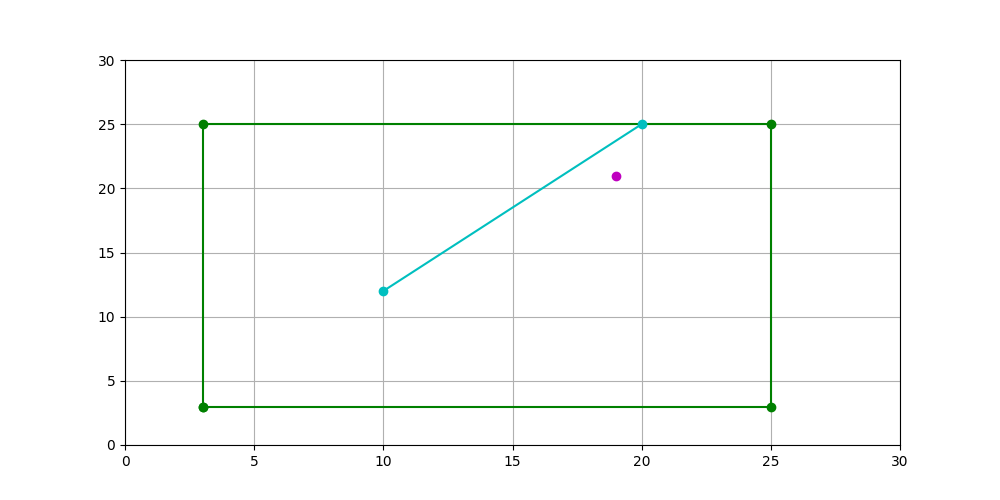
\includegraphics[width = 0.6\linewidth]{Figure-2D}
    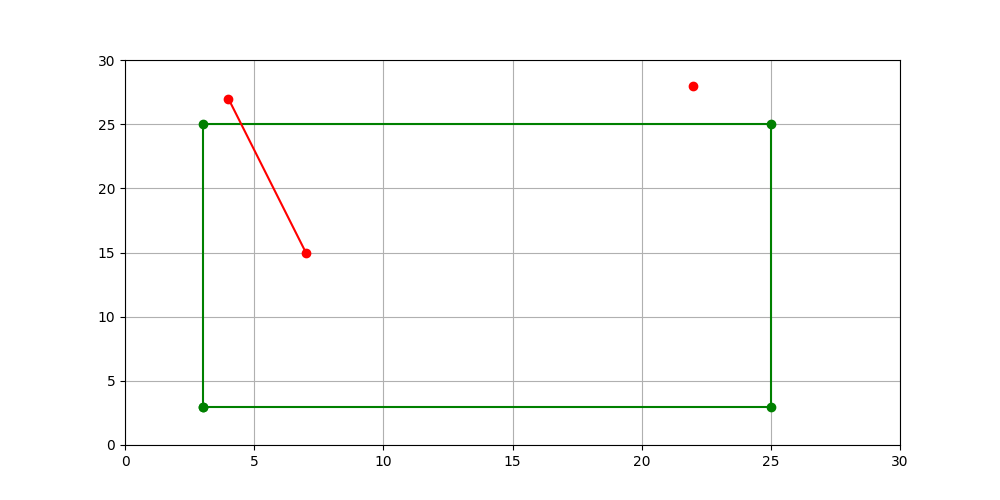
\includegraphics[width = 0.6\linewidth]{Figure_2D_fuera}
\end{itemize}
\end{frame}

\begin{frame}{Programación 2-D}
 \begin{itemize}
  \item Como se puede ver en las imágenes anteriores el rectángulo 2-D generado pinta de color morado el punto al reconocer que se encuentra dentro de la figura. Por otro lado, al encontrarse fuera de la figura se pinta de color rojo el punto.
  \item También se puede ver en la imagen que se genera un segmento donde se utiliza la misma propuesta para reconocer si esta dentro o fuera de la figura.
  \item Para que la figura reconozca que el segmento se encuentra dentro de la figura ambos puntos se tienen que encontrar dentro de la figura y por consiguiente se pinta de color celeste, caso contrario, se pinta de color rojo el segmento completo.
 \end{itemize}
\end{frame}

\begin{frame}{Programación 3-D}
 \begin{itemize}
  \item Una vez realizada la programación en 2-D se extrapolo las mismas funciones y se genero una figura en 3-D.
  
  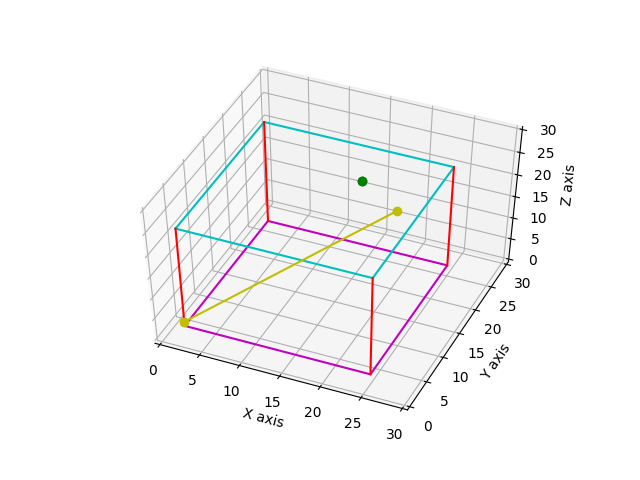
\includegraphics[width=0.6\linewidth]{Figure_3-D_dentro}
 \end{itemize}
\end{frame}

\begin{frame}{Programación 3-D}
  \begin{itemize}
   \item (Misma figura generada con fines de prueba)
  \end{itemize}
  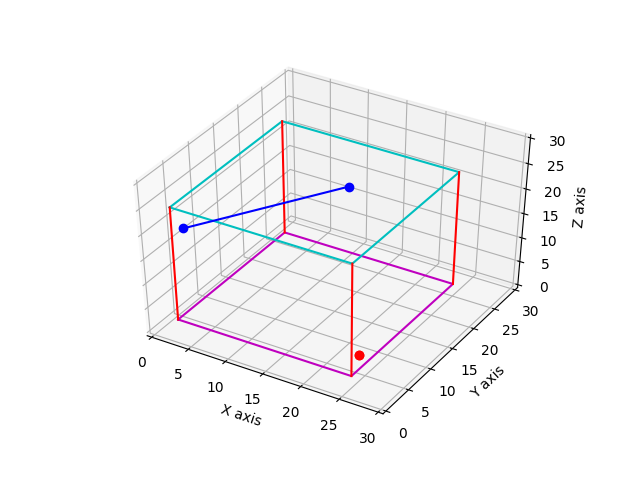
\includegraphics[width=0.6\linewidth]{Figure_3-D_fuera}
\end{frame}

\begin{frame}{Programación 3-D}
  \begin{itemize}
   \item Como se puede ver en las imágenes anteriores al reconocer si el punto o el segmento se encuentran dentro de la imagen se pintan de color verde y amarillo respectivamente, caso contrario, el punto y el segmentos pintan de color rojo y azul respectivamente.
   \item Para reconocer si el segmento esta dentro de la figura, ambos puntos en los tres ejes tienen que estar dentro de la figura en 3-D.
  \end{itemize}
\end{frame}


\begin{frame}{Problemas}
  \begin{itemize}
   \item Para detectar si el segmento se encuentra dentro de la figura se tiene una variable 's' que se utiliza en los cálculos finales de la propuesta, no se entendió que representaba.
  \end{itemize}
\end{frame}

\begin{frame}{ToDo}
  \begin{itemize}
   \item Identificar para que se utiliza la variable 's' dentro de la ecuación de detección.
   \item Detectar la cara por la cual ingresa el segmento.
  \end{itemize}
\end{frame}


\medskip
\bibliographystyle{plain}
\bibliography{/home/yerkozec/Desktop/pt/memoria/Referencia}

\end{document}
